\documentclass[12pt, a4paper]{article}

% ── Encodage et langue ──────────────────────────────────────────────────────
\usepackage[utf8]{inputenc}
\usepackage[T1]{fontenc}
\usepackage[french]{babel}

% ── Mise en page ────────────────────────────────────────────────────────────
\usepackage[top=2.5cm, bottom=2.5cm, left=2.8cm, right=2.8cm]{geometry}
\usepackage{setspace}
\onehalfspacing

% ── Mathématiques ───────────────────────────────────────────────────────────
\usepackage{amsmath, amssymb, amsthm}
\usepackage{mathtools}
\usepackage{bbm}          % \mathbbm{1}
\usepackage{dsfont}       % \mathds{1}

% ── Théorèmes ───────────────────────────────────────────────────────────────
\newtheorem{theorem}{Théorème}[section]
\newtheorem{proposition}[theorem]{Proposition}
\newtheorem{lemma}[theorem]{Lemme}
\newtheorem{corollary}[theorem]{Corollaire}
\theoremstyle{definition}
\newtheorem{definition}[theorem]{Définition}
\newtheorem{example}[theorem]{Exemple}
\newtheorem{remark}[theorem]{Remarque}

% ── Algorithmes ─────────────────────────────────────────────────────────────
\usepackage[ruled, vlined, french]{algorithm2e}

% ── Figures et tableaux ─────────────────────────────────────────────────────
\usepackage{graphicx}
\usepackage{float}
\usepackage{subcaption}
\usepackage{booktabs}
\usepackage{caption}

% ── Couleurs et hyperliens ──────────────────────────────────────────────────
\usepackage{xcolor}
\usepackage[colorlinks=true, linkcolor=blue!70!black,
            citecolor=blue!70!black, urlcolor=blue!70!black]{hyperref}

% ── Bibliographie ───────────────────────────────────────────────────────────
\usepackage[numbers, sort&compress]{natbib}

% ── Raccourcis mathématiques ────────────────────────────────────────────────
\newcommand{\R}{\mathbb{R}}
\newcommand{\N}{\mathbb{N}}
\newcommand{\E}{\mathbb{E}}
\newcommand{\Prob}{\mathbb{P}}
\newcommand{\Zcal}{\mathcal{Z}}
\newcommand{\Fcal}{\mathcal{F}}
\newcommand{\Ncal}{\mathcal{N}}
\newcommand{\norm}[1]{\left\|#1\right\|}
\newcommand{\abs}[1]{\left|#1\right|}
\newcommand{\inner}[2]{\langle #1,\, #2 \rangle}
\newcommand{\Id}{\mathrm{Id}}
\newcommand{\Tr}{\mathrm{Tr}}
\DeclareMathOperator*{\argmin}{arg\,min}
\DeclareMathOperator*{\argmax}{arg\,max}

% —— Figures —————————————————————————————————————————————————————————————————
\graphicspath{{figures/}}

% ════════════════════════════════════════════════════════════════════════════
\begin{document}

% ── Page de titre ───────────────────────────────────────────────────────────
\begin{titlepage}
    \begin{center}

        {\Large Université Paris Cité \\[0.3em]
        M1 Mathématiques, Modélisation et Apprentissage Statistique} \\[1.5em]

        \rule{\textwidth}{0.4pt}

        \vspace{4em}

        {\huge\bfseries Estimation dans un problème inverse linéaire
        à variables cachées :\\[0.6em]
        \large vraisemblance, algorithme EM\\[0.2em]
        et analyse de l'erreur \par}

        \vspace{5em}

        {\Large Arthur Conche, Abdel Niang} \\[1em]
        {\Large Année universitaire 2025--2026} \\[6em]

        \textbf{Responsable universitaire :} Camille Pouchol

    \end{center}
\end{titlepage}

% ── Remerciements ───────────────────────────────────────────────────────────
\newpage
\begin{center}
    {\Large Remerciements}
\end{center}
\vspace{0.5em}
\noindent\rule{\textwidth}{1pt}
\vspace{1em}

% TODO : rédiger les remerciements

\vspace{1em}
\noindent\rule{\textwidth}{1pt}

% ── Résumé ──────────────────────────────────────────────────────────────────
\newpage
\begin{abstract}
% TODO : rédiger le résumé (environ 15 lignes)
% Présenter brièvement : le modèle (M), les deux cas d'application,
% les méthodes étudiées (MV directe, EM), l'analyse de l'erreur.
\end{abstract}

% ── Table des matières ──────────────────────────────────────────────────────
\newpage
\tableofcontents

% ════════════════════════════════════════════════════════════════════════════
\newpage
\section*{Introduction}
\addcontentsline{toc}{section}{Introduction}
\label{sec:introduction}

La détermination de la structure tridimensionnelle des macromolécules biologiques
--- protéines, virus, complexes ribosomaux --- est l'une des questions centrales
de la biologie structurale moderne. Comprendre la géométrie précise d'une protéine,
c'est comprendre son fonctionnement, ses interactions avec d'autres molécules, et
ouvrir la voie à la conception rationnelle de médicaments. Depuis les années 2010,
la \textit{cryo-microscopie électronique} (cryo-EM) s'est imposée comme la technique
de référence pour cette reconstruction, au point que ses pionniers, Jacques Dubochet,
Joachim Frank et Richard Henderson, ont reçu le Prix Nobel de Chimie en 2017.

Le principe de la cryo-EM est le suivant. Des milliers de copies identiques de la
molécule d'intérêt sont plongées dans une solution rapidement vitrifiée, si bien que
chaque copie se fige dans une orientation aléatoire. Un faisceau d'électrons traverse
l'échantillon et produit, pour chaque copie, une image bidimensionnelle : c'est la
projection de la molécule selon l'axe du faisceau. L'observateur dispose donc de
$n$ images, chacune étant la projection d'une molécule ayant subi une rotation
inconnue dans $SO(3)$, et fortement perturbée par le bruit de mesure inhérent à la
technique. La question est alors : comment reconstruire la structure 3D originale
à partir de ces projections bruitées dont les orientations sont toutes ignorées ?

Ce problème appartient à la classe des \textit{problèmes inverses linéaires avec
variables cachées}. Dans la modélisation mathématique, la structure moléculaire
inconnue est représentée par un paramètre $\theta$ dans un espace fonctionnel
approprié. Chaque rotation aléatoire $Z_i$, non observée, détermine un opérateur
linéaire $A_{Z_i}$ qui projette $\theta$ en une image bruitée $Y_i = A_{Z_i}\theta
+ \sigma E_i$. La difficulté fondamentale est double : il faut estimer $\theta$
sans connaître les $Z_i$, et la marginalisation sur ces variables cachées rend la
vraisemblance non quadratique, invalidant les approches classiques des moindres carrés.

Ce rapport étudie ce problème dans deux cas simplifiés qui en capturent les
difficultés essentielles. Le premier cas, en dimension 1, porte sur des translations
aléatoires d'un signal périodique : il est analytiquement tractable et sert de
terrain d'expérimentation pour tous les développements théoriques et numériques.
Le second cas, en dimension 2, est l'analogue direct de la cryo-EM : des rotations
aléatoires dans $\mathbb{R}^2$ suivies d'une projection, ce qui correspond à la
transformée de Radon en deux dimensions.

Nous commençons par poser rigoureusement le cadre mathématique et les deux cas
d'application (Section~\ref{sec:mise_en_place}). Pour forger l'intuition, nous
résolvons intégralement le problème simplifié où les transformations sont connues et
constantes, ce qui fournit un estimateur explicite et une borne d'erreur de référence
(Section~\ref{sec:sans_cachees}). Nous formulons ensuite le problème de maximum de
vraisemblance dans le cas général et mettons en évidence une difficulté d'identifiabilité
qui impose de reconsidérer la mesure d'erreur usuelle
(Section~\ref{sec:mle}). Deux algorithmes d'optimisation sont alors développés et
comparés : une descente de gradient directe sur la log-vraisemblance et l'algorithme
d'espérance-maximisation (EM), dont chaque itération se ramène à un problème
quadratique convexe (Section~\ref{sec:optimisation}). Nous analysons enfin
quantitativement la précision de l'estimation en fonction du nombre de données $n$
et du niveau de bruit $\sigma$, dans le cas avec variables cachées
(Section~\ref{sec:analyse_erreur}), avant de présenter des extensions vers le cas
des rotations en 2D et des approches de régularisation
(Section~\ref{sec:extensions}).

\section{Mise en place du problème}
\label{sec:mise_en_place}

\subsection{Cadre général}
\label{subsec:cadre_general}

On dispose de $n$ observations $Y_1, \ldots, Y_n \in \mathbb{R}^p$ et l'on cherche
à estimer un paramètre inconnu $\theta$ appartenant à $E$, espace de Hilbert
de dimension finie muni du produit scalaire $\inner{\cdot}{\cdot}$.

Soit $(\Zcal, \Fcal, \mu)$ un espace mesuré. Pour chaque $z \in \Zcal$, on se
donne un opérateur linéaire borné $A_z \in L(E, \R^p)$. Les observations suivent
le modèle
\begin{equation}
    Y_i = A_{Z_i}\theta + \sigma E_i, \qquad i \in \{1, \ldots, n\}, \tag{M}
    \label{eq:modele}
\end{equation}
où $\sigma > 0$ est un niveau de bruit connu, et les variables aléatoires
$(Z_i)_{1 \leq i \leq n}$ et $(E_i)_{1 \leq i \leq n}$ vérifient les hypothèses suivantes.

\begin{itemize}
    \item Les $(Z_i)_{1 \leq i \leq n}$, à valeurs dans $\Zcal$, sont i.i.d.\
    de densité $f_Z$ par rapport à la mesure $\mu$.
    \item Les $(E_i)_{1 \leq i \leq n}$, à valeurs dans $\R^p$, sont i.i.d.\
    de loi $\Ncal(0, \mathrm{Id}_p)$.
    \item Les familles $(Z_i)_{1 \leq i \leq n}$ et $(E_i)_{1 \leq i \leq n}$
    sont indépendantes.
\end{itemize}

Les variables $(Z_i)$ jouent le rôle de \textit{variables cachées} : elles
déterminent quelle transformation linéaire $A_{Z_i}$ est appliquée à $\theta$
avant observation, mais elles ne sont pas accessibles à l'observateur.
Chaque $Y_i$ est donc une version transformée et bruitée de $\theta$, dont
la transformation elle-même est inconnue. C'est cette double incertitude ---
sur $\theta$ et sur les $Z_i$ --- qui constitue la difficulté centrale du problème.
% - Espace de Hilbert E, espace mesuré (Z, F, mu)
% - Opérateurs A_z in L(E, R^p)
% - Présentation du modèle (M) : Y_i = A_{Z_i} theta + sigma E_i
% - Hypothèses : Z_i i.i.d. de densité f_Z, E_i ~ N(0, Id_p), indépendance

\subsection{Cas d'application}
\label{subsec:cas_application}

\subsubsection{Cas 1 : translations en 1D}
\label{subsubsec:cas1}

Le premier cas d'application est celui des \textit{translations sur le tore}.
On note $\mathbb{T} = \mathbb{R} / 2\pi\mathbb{Z}$ le tore unidimensionnel,
que l'on identifie à l'intervalle $[0, 2\pi)$ muni de la mesure de Lebesgue.
L'espace ambiant est $L^2(\mathbb{T})$, l'espace des fonctions de carré intégrable
et $2\pi$-périodiques, muni du produit scalaire
\[
    \inner{f}{g} = \frac{1}{2\pi} \int_0^{2\pi} f(x)\,\overline{g(x)}\,\mathrm{d}x.
\]

\paragraph{Sous-espace $E$ et discrétisation.}
On travaille avec un sous-espace de dimension finie $d$ de $L^2(\mathbb{T})$,
engendré par les premières harmoniques de Fourier :
\[
    E = \mathrm{Vect}\!\left(x \mapsto e^{ikx},\;
    -\frac{d-1}{2} \leq k \leq \frac{d-1}{2}\right),
\]
où $d$ est supposé impair pour que l'espace soit symétrique autour de la fréquence
nulle. Tout $\theta \in E$ s'écrit donc comme un polynôme trigonométrique de degré
au plus $\frac{d-1}{2}$.
En pratique numérique, comme $\theta$ est à valeurs réelles, la condition
$\hat\theta_{-k} = \overline{\hat\theta_k}$ permet de se ramener à la base réelle
$\bigl\{1,\,\cos(kx),\,\sin(kx)\bigr\}_{k=1}^{N}$ (avec $N = (d-1)/2$) et de
représenter $\theta$ par un vecteur de coefficients
$u = (a_0, a_1, b_1, \ldots, a_N, b_N)^\top \in \R^d$ via
\[
    \theta(x) = a_0 + \sum_{k=1}^{N}\bigl(a_k\cos(kx) + b_k\sin(kx)\bigr).
\]
C'est cette paramétrisation réelle qu'on utilise dans les implémentations numériques.

Les observations sont effectuées sur une grille uniforme de $p \geq d$ points :
\[
    x_j = 2\pi\,\frac{j}{p}, \qquad j \in \{0, \ldots, p-1\}.
\]
La condition $p \geq d$ garantit que l'évaluation sur la grille est injective
sur $E$, ce qui est nécessaire pour l'identifiabilité du problème.

\paragraph{Opérateur de translation.}
L'espace des variables cachées est $\Zcal = [0, 2\pi)$ muni de la mesure de
Lebesgue normalisée. Pour $z \in [0, 2\pi)$ et $\theta \in E$, l'opérateur
$A_z \in L(E, \R^p)$ est défini par évaluation de la translatée de $\theta$ :
\[
    (A_z\theta)_j = \theta(x_j - z), \qquad j \in \{0, \ldots, p-1\},
\]
où la soustraction $x_j - z$ est entendue modulo $2\pi$. Autrement dit, $A_z\theta$
est le vecteur des valeurs de $\theta$ décalé de $z$ sur la grille.

\begin{remark}
    Puisque $\theta \in E$ est un polynôme trigonométrique, sa translatée
    $x \mapsto \theta(x - z)$ appartient encore à $E$ pour tout $z \in [0, 2\pi)$.
    L'opérateur $A_z$ est donc bien défini et sa structure se lit aisément dans la
    base de Fourier : si $\theta = \sum_k \hat{\theta}_k\, e^{ikx}$, alors
    \[
        (A_z\theta)_j = \sum_{k} \hat{\theta}_k\, e^{ik(x_j - z)}
        = \sum_{k} \hat{\theta}_k\, e^{-ikz}\, e^{ikx_j}.
    \]
    La translation par $z$ agit donc comme une modulation de phase dans l'espace de
    Fourier : le coefficient $\hat{\theta}_k$ est multiplié par $e^{-ikz}$.
\end{remark}

\paragraph{Modèle dans le Cas 1.}
Le modèle~\eqref{eq:modele} se spécialise ici en
\[
    Y_i = A_{Z_i}\theta + \sigma E_i \in \R^p,
    \qquad (Y_i)_j = \theta(x_j - Z_i) + \sigma\,(E_i)_j,
\]
où les $Z_i$ sont i.i.d. de loi uniforme sur $[0, 2\pi)$, et les $(E_i)_j$
sont i.i.d. $\Ncal(0, 1)$. Chaque observation $Y_i$ est donc un échantillonnage
bruité de $\theta$ sur la grille, après une translation aléatoire inconnue.
L'objectif est de reconstruire $\theta$ à partir des $n$ vecteurs $Y_1, \ldots, Y_n$,
sans connaître les décalages $Z_1, \ldots, Z_n$.

\paragraph{Lien avec la cryo-EM.}
Ce cas constitue l'analogue unidimensionnel du problème de reconstruction
moléculaire décrit en introduction. Le signal $\theta$ joue le rôle de la structure
à reconstruire, la translation aléatoire $Z_i$ simule l'orientation inconnue de la
molécule, et la projection sur la grille correspond à l'acquisition d'une image
discrétisée. Sa relative simplicité analytique --- notamment la diagonalisation
de $A_z$ dans la base de Fourier --- en fait le terrain naturel pour développer
et valider les méthodes d'estimation étudiées dans ce rapport.

\subsubsection{Cas 2 : rotations et projections en 2D}
\label{subsubsec:cas2}

Le second cas d'application est celui des \textit{rotations et projections en
dimension 2}. Il constitue l'analogue bidimensionnel direct du problème de
reconstruction en cryo-EM, et est étroitement lié à la tomographie par rayons X.

\paragraph{Espace fonctionnel.}
On note $B(0,1) = \{(x,y) \in \R^2 : x^2 + y^2 \leq 1\}$ la boule unité
euclidienne dans $\R^2$. L'espace ambiant est $L^2(B(0,1))$, muni du produit
scalaire
\[
    \inner{f}{g} = \int_{B(0,1)} f(\mathbf{x})\,\overline{g(\mathbf{x})}\,\mathrm{d}\mathbf{x}.
\]
Le paramètre inconnu $\theta \in E$, où $E$ est un sous-espace de dimension
finie $d$ de $L^2(B(0,1))$, représente la densité bidimensionnelle à reconstruire
--- l'analogue discret de la densité électronique d'une molécule.

\paragraph{Opérateur de rotation.}
L'espace des variables cachées est $\Zcal = [0, 2\pi)$ muni de la mesure de
Lebesgue normalisée. Pour $z \in [0, 2\pi)$, on note $R_z$ la rotation plane
d'angle $z$, de matrice
\[
    R_z = \begin{pmatrix} \cos z & -\sin z \\ \sin z & \cos z \end{pmatrix}.
\]
L'action de $R_z$ sur une fonction $\theta \in L^2(B(0,1))$ est définie par
composition :
\[
    (R_z\theta)(\mathbf{x}) = \theta(R_z^{-1}\mathbf{x}) = \theta(R_{-z}\mathbf{x}),
    \qquad \mathbf{x} \in B(0,1).
\]
Puisque $R_z$ est une isométrie de $B(0,1)$ dans lui-même, $R_z\theta$ est bien
dans $L^2(B(0,1))$ dès que $\theta$ l'est.

\paragraph{Opérateur de projection.}
On définit l'opérateur de projection $P : L^2(B(0,1)) \to L^2([-1,1])$ par
intégration selon l'axe $y$ :
\[
    (P\theta)(x) = \int_{\R} \theta(x, y)\,\mathrm{d}y, \qquad x \in [-1, 1].
\]
Cet opérateur est la \textit{transformée de Radon} de $\theta$ selon la direction
verticale : il donne la somme (intégrale) de $\theta$ le long de chaque droite
verticale $\{x\} \times \R$.

\begin{remark}
    La transformée de Radon complète de $\theta$ consiste à calculer $P(R_z\theta)$
    pour tous les angles $z \in [0, \pi)$, ce qui correspond à projeter $\theta$ selon
    toutes les directions du plan. Le théorème de la tranche de Fourier établit que la
    transformée de Fourier 1D de $P(R_z\theta)$ en $x$ coïncide avec la transformée
    de Fourier 2D de $\theta$ restreinte à la droite de direction $z$. C'est le
    fondement théorique des algorithmes de rétroprojection filtrée utilisés en
    tomographie.
\end{remark}

\paragraph{Opérateur $A_z$ et discrétisation.}
L'opérateur $A_z \in L(E, \R^p)$ combine la rotation et la projection :
\[
    A_z = \mathrm{ev}_{\text{grille}} \circ\, P \circ R_z,
\]
où $\mathrm{ev}_{\text{grille}}$ désigne l'évaluation sur une grille uniforme
de $p$ points $x_j = j/p \in [0, 1]$, $j \in \{0, \ldots, p-1\}$. Explicitement :
\[
    (A_z\theta)_j = (P R_z\theta)(x_j) = \int_{\R} \theta\!\left(R_{-z}
    \begin{pmatrix} x_j \\ y \end{pmatrix}\right)\mathrm{d}y,
    \qquad j \in \{0, \ldots, p-1\}.
\]
Chaque observation $(A_z\theta)_j$ est donc la valeur en $x_j$ de la projection
de $\theta$ après rotation d'angle $z$.

\paragraph{Modèle dans le Cas 2.}
Le modèle~\eqref{eq:modele} se spécialise en
\[
    Y_i = A_{Z_i}\theta + \sigma E_i \in \R^p, \qquad
    (Y_i)_j = \int_{\R} \theta\!\left(R_{-Z_i}\begin{pmatrix}x_j\\y\end{pmatrix}\right)
    \mathrm{d}y + \sigma\,(E_i)_j,
\]
où les $Z_i$ sont i.i.d. de loi uniforme sur $[0, 2\pi)$, et les $(E_i)_j$ sont
i.i.d. $\Ncal(0,1)$. Chaque $Y_i$ est un sinogramme partiel bruité de $\theta$ :
c'est la projection de $\theta$ selon une direction aléatoire inconnue,
échantillonnée sur $p$ points.

\paragraph{Comparaison avec le Cas 1.}
Le Cas 2 est structurellement plus proche du problème physique de départ que
le Cas 1. Le groupe des variables cachées est le même ($[0, 2\pi)$ dans les deux
cas), mais l'opérateur $A_z$ est ici un opérateur intégral --- la composition
d'une rotation et d'une projection --- là où il était simplement une évaluation
décalée dans le Cas 1. La diagonalisation dans la base de Fourier n'est plus
aussi directe, ce qui rend les développements analytiques plus délicats et les
algorithmes d'estimation plus coûteux numériquement. Pour ces raisons, le Cas 2
sera traité principalement en Section~\ref{sec:extensions}, après que les méthodes
aient été développées et validées sur le Cas 1.

\subsection{Simulation des données et premières observations numériques}
\label{subsec:simulation}
% - Choix d'un sous-espace raisonnable de L^2(T), dimension d
% - Génération des données du Cas 1 pour différents sigma, d, p
% - Premières visualisations : impact du bruit, du nombre de mesures
\paragraph{Génération d'une observation dans le Cas 1.}
Pour simuler une observation $Y_i$, on fixe d'abord le vecteur $u \in \mathbb{R}^d$ des 
coordonnées de $\theta$ dans la base trigonométrique réelle. 
On tire un $Z_i$ à valeur dans $[0, 2 \pi]$ et on évalue $\theta$ translatée de $Z_i$ en chaque point de 
la grille $x_j = 2 \pi \frac{j}{p}, j \in \{0,\dots, p-1\}$.
On tire ensuite un vecteur de bruit gaussien $E_i \sim \mathcal{N}(0, \sigma \mathbf{Id}_p)$,
et on observe $(Y_i)_j = \theta(x_j - Z_i) + (E_i)_j$.


\begin{figure}[H]
    \centering
    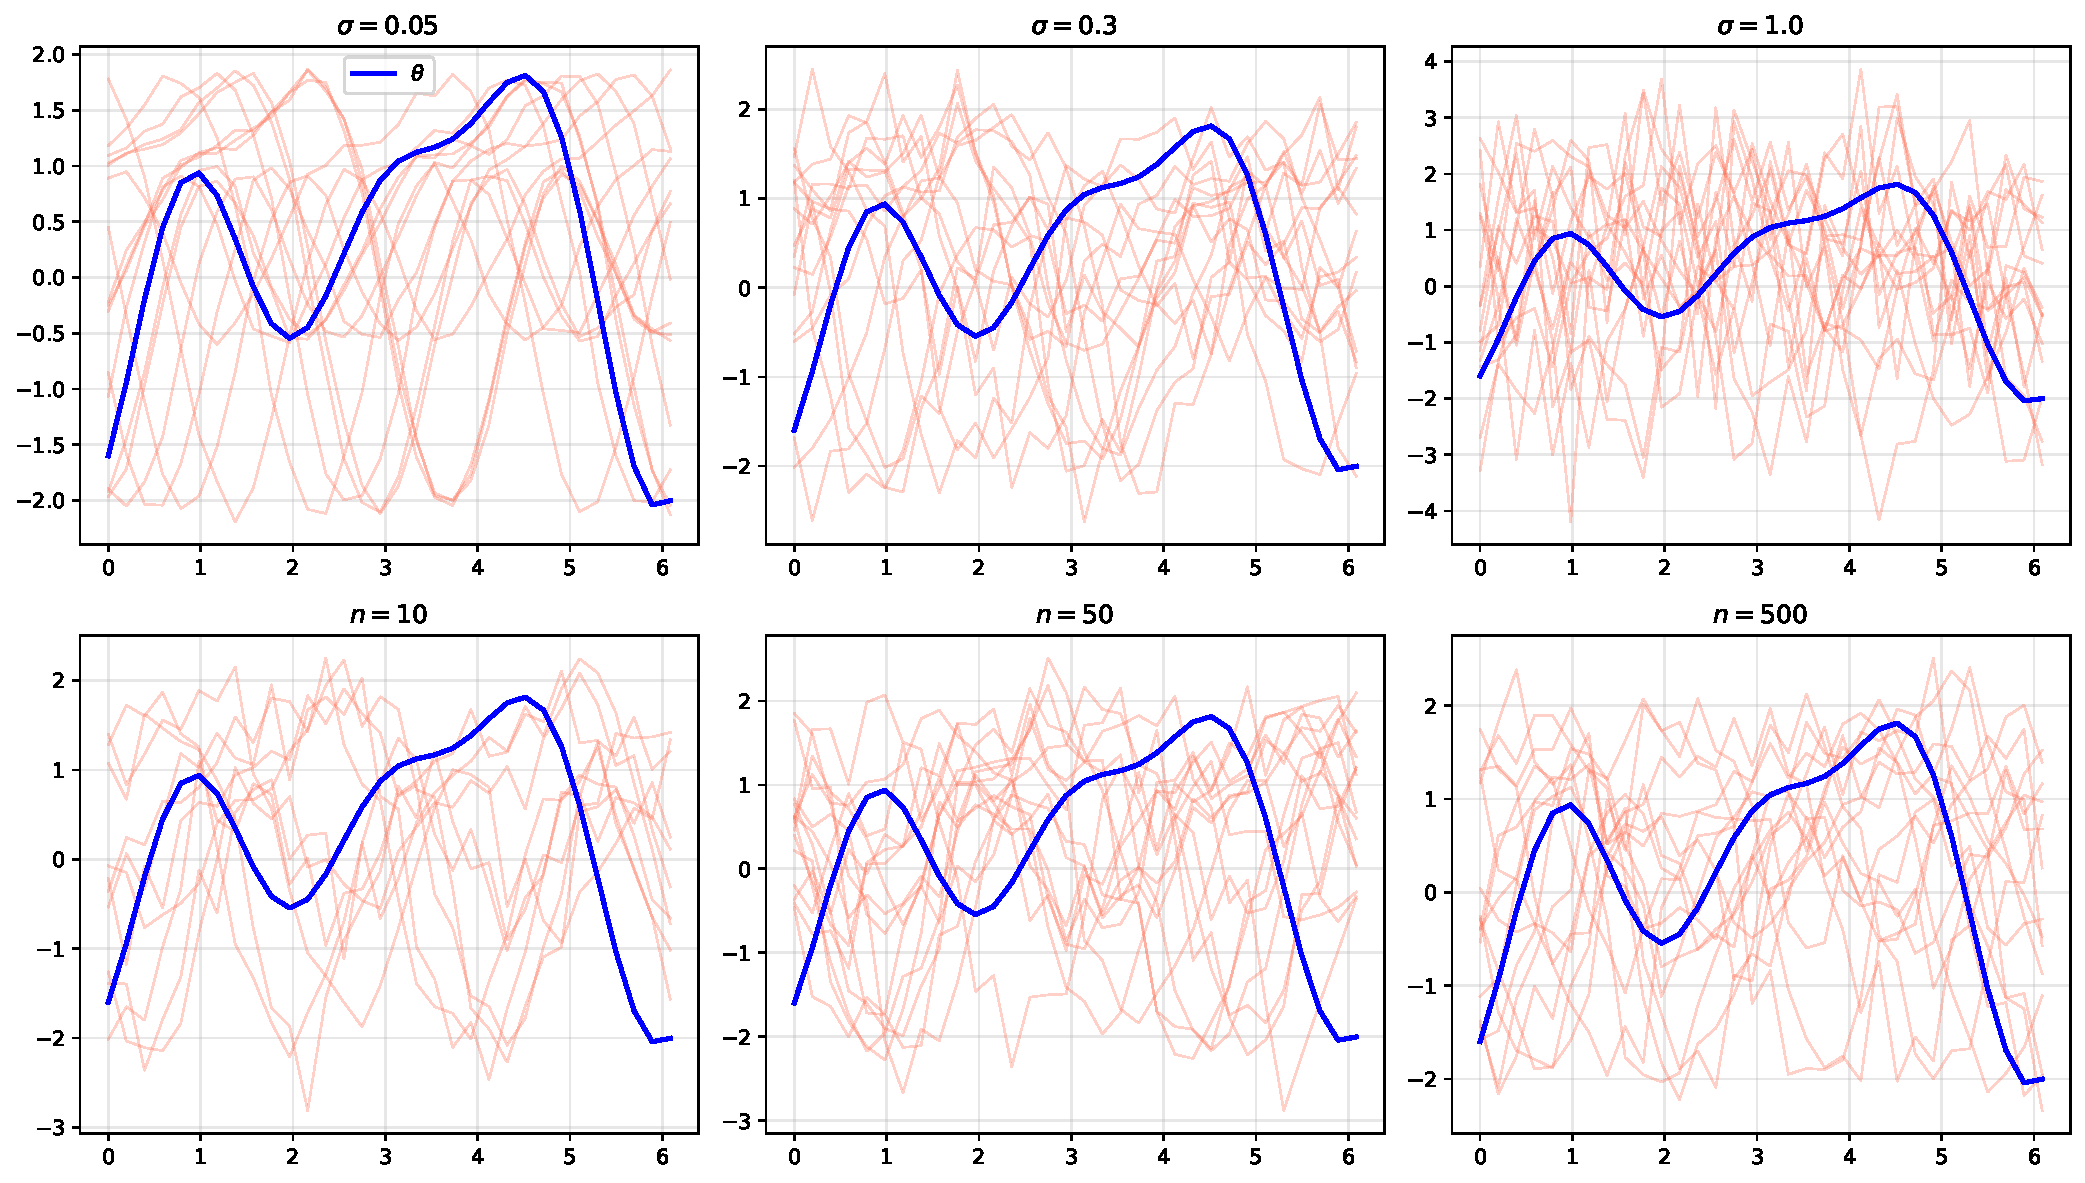
\includegraphics[width=\textwidth]{simulation_parametres.pdf}
    \caption{Influence des paramètres sur les observations simulées.
    Haut : effet du niveau de bruit $\sigma$.
    Bas : effet du nombre d'observations $n$.}
    \label{fig:simulation_parametres}
\end{figure}


% ════════════════════════════════════════════════════════════════════════════
\newpage
\section{Cas de référence : le modèle sans variables cachées}
\label{sec:sans_cachees}
% Objectif de cette section : résoudre complètement le problème simplifié A_z = A
% pour tous les z. Tout est explicite ici — cela sert de référence et de motivation
% pour mesurer la difficulté introduite par les variables cachées dans les sections suivantes.

\subsection{Modèle simplifié et estimateur du maximum de vraisemblance}
\label{subsec:modele_simplifie}
% - Hypothèse : A_z = A pour tout z, avec A^T A inversible
% - Le modèle devient : Y_i = A theta + sigma E_i
% - Densité de Y_i : gaussienne N(A theta, sigma^2 Id_p)
% - Log-vraisemblance : explicite, quadratique en theta
% - Estimateur MV : theta_hat_n = (A^T A)^{-1} A^T * (1/n) sum Y_i

\subsection{Convexité et résolution exacte}
\label{subsec:convexite_simple}
% - La log-vraisemblance négative est strictement convexe (car A^T A inversible)
% - Solution explicite du problème d'optimisation : pas besoin d'algorithme itératif
% - Interprétation géométrique : projection orthogonale sur Im(A)

\subsection{Analyse de l'erreur d'estimation}
\label{subsec:erreur_simple}
% - Calcul de epsilon_n(sigma) = E[|| theta_hat_n - theta ||^2]^{1/2}
% - Preuve : epsilon_n = (sigma / sqrt(n)) * sqrt(Tr((A^T A)^{-1}))
% - Nombre minimal de données n pour avoir epsilon_n <= epsilon (epsilon > 0 donné)
% - Discussion : rôle de sigma, de la dimension de E, de la structure de A

\subsection{Ce que ce cas enseigne sur le cas général}
\label{subsec:lecons}
% - Quand A_z varie avec z, l'estimateur explicite n'existe plus
% - L'intégration sur les Z_i cachés rend la vraisemblance non quadratique
% - Motivation pour les algorithmes itératifs des sections suivantes


% ════════════════════════════════════════════════════════════════════════════
\newpage
\section{Formulation variationnelle et maximum de vraisemblance}
\label{sec:mle}

\subsection{Densité du couple \texorpdfstring{$(Y, Z)$}{(Y,Z)} et vraisemblance marginale}
\label{subsec:densite}
% - Densité conditionnelle de Y | Z=z : gaussienne N(A_z theta, sigma^2 Id_p)
% - Densité jointe (Y, Z) par rapport à lambda_p x mu
% - Vraisemblance marginale : intégration sur Z -> L(theta ; Y_1,...,Y_n)
% - Log-vraisemblance : somme de log-somexp

\subsection{Propriétés analytiques de la log-vraisemblance}
\label{subsec:proprietes_ll}
% - Régularité (différentiabilité, gradient, hessien)
% - Convexité : la fonction à minimiser est-elle convexe ? Justification

\subsection{Identifiabilité et choix d'une métrique adaptée}
\label{subsec:identifiabilite}
% - Pourquoi la norme standard || theta_hat - theta || est inadaptée (Cas 1)
% - Invariance par translation : L(A_z theta) = L(A_z vartheta) pour certains theta != vartheta
% - Reformulation : epsilon_n^2 = E[ inf_{L(A_z vartheta)=L(A_z theta)} || theta_hat - vartheta ||^2 ]
% - Dans le Cas 1 : simplification avec inf_{a in [0,2pi]} || tau_a theta_hat - vartheta ||^2


% ════════════════════════════════════════════════════════════════════════════
\newpage
\section{Résolution du problème d'optimisation}
\label{sec:optimisation}

\subsection{Approche directe : descente de gradient}
\label{subsec:gradient}
% - Calcul du gradient de la log-vraisemblance négative
% - Algorithme de gradient à pas fixe / pas décroissant
% - Analyse de la convergence (conditions suffisantes)
% - Implémentation et résultats numériques (Cas 1)

\subsection{Algorithme Espérance-Maximisation}
\label{subsec:em}

\subsubsection{Principe général}
\label{subsubsec:em_general}
% - Données complètes vs données incomplètes
% - Décomposition de la log-vraisemblance : identité de Fisher
% - Étape E : calcul de Q(theta | theta^(k)) = E_{Z|Y,theta^(k)}[log p(Y,Z;theta)]
% - Étape M : theta^(k+1) = argmax_theta Q(theta | theta^(k))
% - Propriété fondamentale : croissance monotone de la vraisemblance

\subsubsection{Application au modèle (M)}
\label{subsubsec:em_modele}
% - Calcul explicite de Q(theta | theta^(k)) pour le modèle (M)
% - Montrer que l'étape M est un problème quadratique convexe
% - Forme explicite de la solution (système linéaire)
% - Implémentation et résultats numériques (Cas 1)

\subsection{Comparaison des deux approches}
\label{subsec:comparaison}
% - Complexité par itération : gradient vs EM
% - Garanties de convergence : globale vs locale
% - Sensibilité à l'initialisation
% - Résultats numériques croisés : temps de calcul, valeur finale


% ════════════════════════════════════════════════════════════════════════════
\newpage
\section{Analyse de la qualité de l'estimation}
\label{sec:analyse_erreur}

\subsection{Retour au cas général avec variables cachées}
\label{subsec:avec_variables_cachees}
% - Contraste avec la Section 2 : on ne dispose plus d'un estimateur explicite
% - Pourquoi la norme standard || theta_hat - theta || est inadaptée (reprendre Section 3.3)
% - Reformulation de epsilon_n^2(sigma) avec la métrique invariante par translation
% - Dans le Cas 1 : simplification avec inf_{a in [0,2pi]} || tau_a theta_hat - vartheta ||^2

\subsection{Étude numérique de \texorpdfstring{$\varepsilon_n(\sigma)$}{epsilon_n(sigma)}}
\label{subsec:etude_numerique_erreur}
% - Courbes epsilon_n en fonction de n pour différents sigma (Cas 1)
% - Courbes epsilon_n en fonction de sigma pour différents n
% - Impact de d et p : discussion


% ════════════════════════════════════════════════════════════════════════════
\newpage
\section{Extensions}
\label{sec:extensions}

\subsection{Cas 2 : rotations et projections en 2D}
\label{subsec:cas2_extensions}
% - Rappel du modèle, lien avec la tomographie
% - Adaptation des algorithmes (gradient, EM) au Cas 2
% - Résultats numériques : reconstruction d'une image 2D
% - Comparaison avec le Cas 1

\subsection{Régularisation}
\label{subsec:regularisation}
% - Motivation : problème mal posé, connaissance a priori sur theta
% - Ajout d'un terme R(theta) dans la vraisemblance pénalisée
% - Exemples de régulariseurs : Tikhonov (||theta||^2), variation totale, L^1
% - Adaptation des algorithmes : gradient proximal, ADMM
% - Résultats numériques


% ════════════════════════════════════════════════════════════════════════════
\newpage
\section*{Conclusion}
\addcontentsline{toc}{section}{Conclusion}
% - Bilan des méthodes étudiées
% - Apports théoriques et numériques
% - Limites et perspectives


% ── Bibliographie ───────────────────────────────────────────────────────────
\newpage
\bibliographystyle{plainnat}
\bibliography{references}
% Fichier references.bib à créer
% Références suggérées :
%   - Dempster, Laird, Rubin (1977) - article fondateur de l'EM
%   - McLachlan & Krishnan - The EM Algorithm and Extensions
%   - Cavalier (2008) - Inverse problems in statistics
%   - Boyd & Vandenberghe - Convex Optimization (pour la partie optimisation)


\end{document}
